% Politecnico di Milano (PoliMi) - School of Industrial and Information Engineering
%
% Last Revision: October 2021
%
% Copyright 2021 Politecnico di Milano, Italy. NC-BY

\documentclass{Configuration_Files/Template}

%------------------------------------------------------------------------------
%	REQUIRED PACKAGES AND  CONFIGURATIONS
%------------------------------------------------------------------------------

% CONFIGURATIONS
\usepackage{parskip} % For paragraph layout
\usepackage{setspace} % For using single or double spacing
\usepackage{emptypage} % To insert empty pages
\usepackage{multicol} % To write in multiple columns (executive summary)
\setlength\columnsep{15pt} % Column separation in executive summary
\setlength\parindent{0pt} % Indentation
\raggedbottom  

% PACKAGES FOR TITLES
\usepackage{titlesec}
% \titlespacing{\section}{left spacing}{before spacing}{after spacing}
\titlespacing{\section}{0pt}{3.3ex}{2ex}
\titlespacing{\subsection}{0pt}{3.3ex}{1.65ex}
\titlespacing{\subsubsection}{0pt}{3.3ex}{1ex}
\usepackage{color}

% PACKAGES FOR LANGUAGE AND FONT
\usepackage[english]{babel} % The document is in English  
\usepackage[utf8]{inputenc} % UTF8 encoding
\usepackage[T1]{fontenc} % Font encoding
\usepackage[11pt]{moresize} % Big fonts

% PACKAGES FOR IMAGES
\usepackage{graphicx}
\usepackage{transparent} % Enables transparent images
\usepackage{eso-pic} % For the background picture on the title page
\usepackage{subfig} % Numbered and caption subfigures using \subfloat.
\usepackage{tikz} % A package for high-quality hand-made figures.
\usetikzlibrary{}
\graphicspath{{./Images/}} % Directory of the images
\usepackage{caption} % Coloured captions
\usepackage{amsthm,thmtools,xcolor} % Coloured "Theorem"
\usepackage{float}

% STANDARD MATH PACKAGES
\usepackage{amsmath}
\usepackage{amsthm}
\usepackage{amssymb}
\usepackage{amsfonts}
\usepackage{bm}
\usepackage[overload]{empheq} % For braced-style systems of equations.
\usepackage{fix-cm} % To override original LaTeX restrictions on sizes

% PACKAGES FOR TABLES
\usepackage{tabularx}
\usepackage{longtable} % Tables that can span several pages
\usepackage{colortbl}

% PACKAGES FOR ALGORITHMS (PSEUDO-CODE)
\usepackage{algorithm}
\usepackage{algorithmic}

% PACKAGES FOR REFERENCES & BIBLIOGRAPHY
\usepackage[colorlinks=true,linkcolor=black,anchorcolor=black,citecolor=black,filecolor=black,menucolor=black,runcolor=black,urlcolor=black]{hyperref} % Adds clickable links at references
\usepackage{cleveref}
\usepackage[square, numbers, sort&compress]{natbib} % Square brackets, citing references with numbers, citations sorted by appearance in the text and compressed
\bibliographystyle{abbrvnat} % You may use a different style adapted to your field

% OTHER PACKAGES
\usepackage{pdfpages} % To include a pdf file
\usepackage{afterpage}
\usepackage{lipsum} % DUMMY PACKAGE
\usepackage{fancyhdr} % For the headers
\fancyhf{}

% Input of configuration file. Do not change config.tex file unless you really know what you are doing. 
% Define blue color typical of polimi
\definecolor{bluepoli}{cmyk}{0.4,0.1,0,0.4}

% Custom theorem environments
\declaretheoremstyle[
  headfont=\color{bluepoli}\normalfont\bfseries,
  bodyfont=\color{black}\normalfont\itshape,
]{colored}

% Set-up caption colors
\captionsetup[figure]{labelfont={color=bluepoli}} % Set colour of the captions
\captionsetup[table]{labelfont={color=bluepoli}} % Set colour of the captions
\captionsetup[algorithm]{labelfont={color=bluepoli}} % Set colour of the captions

\theoremstyle{colored}
\newtheorem{theorem}{Theorem}[chapter]
\newtheorem{proposition}{Proposition}[chapter]

% Enhances the features of the standard "table" and "tabular" environments.
\newcommand\T{\rule{0pt}{2.6ex}}
\newcommand\B{\rule[-1.2ex]{0pt}{0pt}}

% Pseudo-code algorithm descriptions.
\newcounter{algsubstate}
\renewcommand{\thealgsubstate}{\alph{algsubstate}}
\newenvironment{algsubstates}
  {\setcounter{algsubstate}{0}%
   \renewcommand{\STATE}{%
     \stepcounter{algsubstate}%
     \Statex {\small\thealgsubstate:}\space}}
  {}

% New font size
\newcommand\numfontsize{\@setfontsize\Huge{200}{60}}

% Title format: chapter
\titleformat{\chapter}[hang]{
\fontsize{50}{20}\selectfont\bfseries\filright}{\textcolor{bluepoli} \thechapter\hsp\hspace{2mm}\textcolor{bluepoli}{|   }\hsp}{0pt}{\huge\bfseries \textcolor{bluepoli}
}

% Title format: section
\titleformat{\section}
{\color{bluepoli}\normalfont\Large\bfseries}
{\color{bluepoli}\thesection.}{1em}{}

% Title format: subsection
\titleformat{\subsection}
{\color{bluepoli}\normalfont\large\bfseries}
{\color{bluepoli}\thesubsection.}{1em}{}

% Title format: subsubsection
\titleformat{\subsubsection}
{\color{bluepoli}\normalfont\large\bfseries}
{\color{bluepoli}\thesubsubsection.}{1em}{}

% Shortening for setting no horizontal-spacing
\newcommand{\hsp}{\hspace{0pt}}

\makeatletter
% Renewcommand: cleardoublepage including the background pic
\renewcommand*\cleardoublepage{%
  \clearpage\if@twoside\ifodd\c@page\else
  \null
  \AddToShipoutPicture*{\BackgroundPic}
  \thispagestyle{empty}%
  \newpage
  \if@twocolumn\hbox{}\newpage\fi\fi\fi}
\makeatother

%For correctly numbering algorithms
\numberwithin{algorithm}{chapter}

%----------------------------------------------------------------------------
%	NEW COMMANDS DEFINED
%----------------------------------------------------------------------------

% EXAMPLES OF NEW COMMANDS
\newcommand{\bea}{\begin{eqnarray}} % Shortcut for equation arrays
\newcommand{\eea}{\end{eqnarray}}
\newcommand{\e}[1]{\times 10^{#1}}  % Powers of 10 notation

%----------------------------------------------------------------------------
%	ADD YOUR PACKAGES (be careful of package interaction)
%----------------------------------------------------------------------------

\usepackage{geometry}
\usepackage{tabularx}
\usepackage{booktabs,xltabular}
\usepackage{hyperref}

%----------------------------------------------------------------------------
%	ADD YOUR DEFINITIONS AND COMMANDS (be careful of existing commands)
%----------------------------------------------------------------------------

% Set uniform margins
\geometry{
  left=0.8in,
  right=0.8in,
  top=1in,
  bottom=1in,
  includehead,
  includefoot
}

%----------------------------------------------------------------------------
%	BEGIN OF YOUR DOCUMENT
%----------------------------------------------------------------------------

\begin{document}

\fancypagestyle{plain}{%
\fancyhf{} % Clear all header and footer fields
\fancyhead[RO,RE]{\thepage} %RO=right odd, RE=right even
\renewcommand{\headrulewidth}{0pt}
\renewcommand{\footrulewidth}{0pt}}

%----------------------------------------------------------------------------
%	TITLE PAGE
%----------------------------------------------------------------------------

\pagestyle{empty} % No page numbers
\frontmatter % Use roman page numbering style (i, ii, iii, iv...) for the preamble pages

\puttitle{
    title= ITD Document,
    name= {Mattia Piccinato, Gabriele Puglisi, Jacopo Piazzalunga},
    academicyear= {2023-24},
    link= \href{https://github.com/GabP404/PiazzalungaPiccinatoPuglisi-CodeKataBattle}{Click here}

 }

%----------------------------------------------------------------------------
%	PREAMBLE PAGES: ABSTRACT (inglese e italiano), EXECUTIVE SUMMARY
%----------------------------------------------------------------------------
\startpreamble
\setcounter{page}{1} % Set page counter to 1

%----------------------------------------------------------------------------
%	LIST OF CONTENTS/FIGURES/TABLES/SYMBOLS
%----------------------------------------------------------------------------

% TABLE OF CONTENTS
\thispagestyle{empty}
\tableofcontents % Table of contents 
\thispagestyle{empty}
\cleardoublepage

%-------------------------------------------------------------------------
%	MAIN TEXT
%-------------------------------------------------------------------------.

\addtocontents{toc}{\vspace{2em}} % Add a gap in the Contents, for aesthetics
\mainmatter % Begin numeric (1,2,3...) page numbering


% FIRST CHAPTER
% --------------------------------------------------------------------------
\chapter{Introduction}

\section{Purpose}

This document outlines the implementation and testing procedures that have been followed to develop a functioning prototype of the service described in the ”Requirements Analysis and Specification Document” and ”Design Document”.

{\color{bluepoli}\rule{\linewidth}{0.1pt}}

\subsection{Definitions}

{\color{bluepoli}\rule{\linewidth}{0.1pt}}

\begin{itemize}
\item \textcolor{bluepoli}{Battle:} A Code Kata, that is, a challenge in which teams of players need to solve a problem in a specific coding language and submit their code to get a score according to the rules of the Battle.
\item \textcolor{bluepoli}{Tournament:} A competition composed of many Battles in which participants' overall score is the sum of all the scores obtained in every Battle they participated in, individually or in team with other players.
\item \textcolor{bluepoli}{Student:} The User which takes part into the Tournaments of Battles.
\item \textcolor{bluepoli}{Educator:} The User which organizes Tournaments of Battles to which the Students can participate and who manages every aspect about them.
\item \textcolor{bluepoli}{Consolidation stage:} The Consolidation Stage is the phase of a Battle which starts as soon as the submission deadline expires, during which the Educators who manage the Tournament can eventually assign an additional score to every team, which will be summed to the score previously assigned by the platform.
\end{itemize}

{\color{bluepoli}\rule{\linewidth}{0.1pt}}

\subsection{Acronyms}

{\color{bluepoli}\rule{\linewidth}{0.1pt}}

\begin{itemize}
\item \textcolor{bluepoli}{CK:} Code Kata, that is, a Battle.
\item \textcolor{bluepoli}{CKB:} Code Kata Battle, that is, the name of the platform.
\end{itemize}

{\color{bluepoli}\rule{\linewidth}{0.1pt}}

\section{Revision History}

\noindent
\begin{tabularx}{\textwidth}{llX}
    \toprule
    Revised on & Version & Description \\
    \midrule
    4-Feb-2023 & 1.0 & Initial Release of the document \\
    \bottomrule
\end{tabularx}
\vspace{0.33pt}

{\color{bluepoli}\rule{\linewidth}{0.1pt}}

\section{Reference Documents}

\begin{itemize}
\item \textcolor{bluepoli}{Assignment document A.Y. 2023/2024}\\
(”Requirement Engineering and Design Project: goal, schedule and rules”)
\item \textcolor{bluepoli}{Software Engineering 2 A.Y. 2023/2024 Slides}\\
(Lecture slides provided during the course)
\end{itemize}

{\color{bluepoli}\rule{\linewidth}{0.1pt}}

\section{Document Structure}

This document is composed of six sections:

\begin{itemize}
\item \textcolor{bluepoli}{1st Chapter:} We begin by presenting the problem statement and outlining the system's objectives. We provide essential resources for readers, including definitions and abbreviations, to facilitate a comprehensive understanding of this document.
\item \textcolor{bluepoli}{2nd Chapter:} We present all the functions of the system which the prototype actually implements.
\item \textcolor{bluepoli}{3rd Chapter:} We introduce the programming languages and frameworks we have chosen to embrace, providing comprehensive justifications for each selection.
\item \textcolor{bluepoli}{4th Chapter:} We present the structure of the code.
\item \textcolor{bluepoli}{5th Chapter:} We provide information regarding the testing process, specifically outlining the functions that have undergone testing and elucidating the methodology employed.
\item \textcolor{bluepoli}{6th Chapter:} We offer instructions that comprehensively guide users on installing and running the prototype.
\end{itemize}

{\color{bluepoli}\rule{\linewidth}{0.1pt}}

% SECOND CHAPTER
% --------------------------------------------------------------------------
\chapter{Product functions and requirements}

The CKB platform provides several functions. For every product feature and each requirement outlined in the RASD, we specify whether the prototype incorporates it.

\section{Product functions}

\begin{itemize}
\item \textcolor{bluepoli}{Battles and Tournaments Creation} Educators can create coding challenges (Battles) within Tournaments, specifying details like descriptions, team sizes, deadlines, scoring configurations and, eventually, Badges.
\textcolor{bluepoli}{Implemented} Yes.

\item \textcolor{bluepoli}{Student Participation} On the other hand, Students can join such Tournaments and take part in Battles, individually or in teams.
\textcolor{bluepoli}{Implemented} Yes.

\item \textcolor{bluepoli}{GitHub Integration} The system allows the Students to perform code submissions just by pushing their code on GitHub, thanks to automated workflows triggered by GitHub Actions service.
\textcolor{bluepoli}{Implemented} Yes.

\item \textcolor{bluepoli}{Automated Evaluation} The platform automatically evaluates Student code based on test cases, timeliness, and code quality using external static analysis tools.
\textcolor{bluepoli}{Implemented} Partially. The prototype offers automated functional evaluation exclusively for Java programs. The static analysis has not been implemented.

\item \textcolor{bluepoli}{Scoring and Ranking} It continuously updates team rankings during Battles and provides overall Tournament rankings at the end of each Battle.
\textcolor{bluepoli}{Implemented} Yes.

\item \textcolor{bluepoli}{Badges and Recognition} Educators define Badges which can be obtained by Students, serving as recognition for accomplishments and participation to a certain Tournament.
\textcolor{bluepoli}{Implemented} No. Badges have not been included in the database design.

\item \textcolor{bluepoli}{Manual Optional Evaluation} Educators can manually evaluate Students' work and assign additional scores at the end of every Battle.
\textcolor{bluepoli}{Implemented} Yes.
\end{itemize}

{\color{bluepoli}\rule{\linewidth}{0.1pt}}

\section{Requirements}

{\color{bluepoli}\rule{\linewidth}{0.1pt}}

\begin{enumerate}
    \item[\textcolor{bluepoli}{R1}] The system must allow an unregistered Educator to sign up.
    \textcolor{bluepoli}{Implemented} Yes.
    
    \item[\textcolor{bluepoli}{R2}] The system must allow an unregistered Student to sign up.
    \textcolor{bluepoli}{Implemented} Yes.
    
    \item[\textcolor{bluepoli}{R3}] The system must allow a registered User to log in.
    \textcolor{bluepoli}{Implemented} Yes.
    
    \item[\textcolor{bluepoli}{R4}] The system must allow registered Educators to start the creation process of a Tournament of Code Kata Battles.
    \textcolor{bluepoli}{Implemented} Yes.
    
    \item[\textcolor{bluepoli}{R5}] The system must provide registered Educators of a list of Tournament-related statistics for the Badges definition, during the Tournament creation process.
    \textcolor{bluepoli}{Implemented} No. Badges have not been implemented.
    
    \item[\textcolor{bluepoli}{R6}] The system must provide registered Educators of a specific language which lets them define the Badges, during the Tournament creation process.
    \textcolor{bluepoli}{Implemented} No. Badges have not been implemented.
    
    \item[\textcolor{bluepoli}{R7}] The system must allow registered Educators to grant other registered Educators the permission to manage the Tournament, during the Tournament creation process.
    \textcolor{bluepoli}{Implemented} Yes.
    
    \item[\textcolor{bluepoli}{R8}] The system must allow registered Educators to end the creation process of a Tournament that they started themselves.
    \textcolor{bluepoli}{Implemented} Yes.
    
    \item[\textcolor{bluepoli}{R9}] The system must be able to send notifications to every registered User.
    \textcolor{bluepoli}{Implemented} Yes. The system uses an e-mail service to notify Users.
    
    \item[\textcolor{bluepoli}{R10}] The system must allow a registered Educator to create a Battle in a Tournament if and only if he is the creator of the Tournament or if he was granted the permission to by the latter.
    \textcolor{bluepoli}{Implemented} Yes.
    
    \item[\textcolor{bluepoli}{R11}] The system must allow a registered Student to create a group for a Battle in a Tournament.
    \textcolor{bluepoli}{Implemented} Yes.
    
    \item[\textcolor{bluepoli}{R12}] The system must allow a registered Student to accept an invitation to a group for a Battle in a Tournament.
    \textcolor{bluepoli}{Implemented} Yes.
    
    \item[\textcolor{bluepoli}{R13}] The system must allow registered Students to see the list of ongoing Tournaments and join any of those if its subscription deadline is not expired yet.
    \textcolor{bluepoli}{Implemented} Yes.
    
    \item[\textcolor{bluepoli}{R14}] The system must allow registered Students who are enrolled in a Battle to perform code submissions.
    \textcolor{bluepoli}{Implemented} Yes.
    
    \item[\textcolor{bluepoli}{R15}] The system must be provided of proper APIs to let registered Students perform code submissions through GitHub Actions.
    \textcolor{bluepoli}{Implemented} Yes.
    
    \item[\textcolor{bluepoli}{R16}] The system must update the Battle ranking when a valid code submission is performed.
    \textcolor{bluepoli}{Implemented} Yes.
    
    \item[\textcolor{bluepoli}{R17}] The system must set the Consolidation Stage of a Battle when its submission deadline expires.
    \textcolor{bluepoli}{Implemented} Yes.
    
    \item[\textcolor{bluepoli}{R18}] The system must let Educators to end the Consolidation Stage of a Battle if and only if he is the creator of the Tournament or if he was granted the permission to by the latter.
    \textcolor{bluepoli}{Implemented} Yes.
    
    \item[\textcolor{bluepoli}{R19}] The system must update Tournament ranking when a Battle exits the Consolidation Stage.
    \textcolor{bluepoli}{Implemented} Yes.
    
    \item[\textcolor{bluepoli}{R20}] The system must let Educators who are either the creator of the Tournament or who have been granted the permission to by the latter to close a Tournament if and only if there is no Battle such that either their subscription or submission deadline is not expired yet or such that they are still in the Consolidation Stage.
    \textcolor{bluepoli}{Implemented} Yes.
    
    \item[\textcolor{bluepoli}{R21}] The system must assign an achievements’ Badge for a given Tournament to any Student who satisfied the conditions defined by the creator of the Tournament.
    \textcolor{bluepoli}{Implemented} No. Badges have not been implemented.
    
    \item[\textcolor{bluepoli}{R22}] The system must allow every User to see the Badges which were ever obtained by a given Student.
    \textcolor{bluepoli}{Implemented} No. Badges have not been implemented.
    
    \item[\textcolor{bluepoli}{R23}] The system must notify every registered Student about the creation of a new Tournament.
    \textcolor{bluepoli}{Implemented} Yes.
    
    \item[\textcolor{bluepoli}{R24}] The system must notify every registered Student about the creation of a new Battle within a Tournament they are enrolled in.
    \textcolor{bluepoli}{Implemented} Yes.
    
    \item[\textcolor{bluepoli}{R25}] The system must notify every registered Student about the end of a Battle they are participating in.
    \textcolor{bluepoli}{Implemented} Yes.
    
    \item[\textcolor{bluepoli}{R26}] The system must notify every registered Student about the end of a Tournament they are enrolled in.
    \textcolor{bluepoli}{Implemented} Yes.
    
\end{enumerate}

{\color{bluepoli}\rule{\linewidth}{0.1pt}}

% THIRD CHAPTER
% --------------------------------------------------------------------------
\chapter{Development and frameworks}

\section{Programming Languages}

\subsection{Java}
Java was selected as the backend programming language for our web application due to the following advantages:

\begin{itemize}
    \item \textbf{Platform Independence:} Java's write once, run anywhere (WORA) philosophy allows us to create code that can run on various operating systems without modification, ensuring broad compatibility.
    
    \item \textbf{Robust Ecosystem:} Java boasts a mature and extensive ecosystem, offering a wide range of libraries and frameworks. This rich set of tools provides a solid foundation for building scalable and maintainable backend solutions.
    
    \item \textbf{Community Support:} Java enjoys strong community support, with a vast developer community contributing to its continuous improvement. Regular updates from Oracle enhance the language's reliability and security.
    
    \item \textbf{Object-Oriented Paradigm:} Java's object-oriented programming (OOP) paradigm aligns well with the complexity of web applications. This approach supports the development of modular, extensible, and organized code.
    
    \item \textbf{Readability and Maintainability:} Java emphasizes readability and maintainability, making it conducive to creating backend code that is not only efficient but also easy to manage over the long term.
\end{itemize}

Furthermore, the decision to utilize Java for developing the backend of our prototype was influenced by the chance to implement Spring and JPA frameworks, which we anticipated would expedite the development process.

\subsection{JavaScript}
JavaScript is the standard language used to develop dynamic and interactive web applications. We used it for creating responsive user interfaces and handling client-side scripting for the frontend of out application.

\section{Frameworks}

\subsection{Spring}
The decision to employ the Spring framework for the backend of our application was driven by several advantages:

\begin{itemize}
    \item \textbf{Comprehensive Ecosystem:} Spring provides a comprehensive ecosystem that facilitates the development of robust and scalable applications. Its modular design allows us to selectively use components, enhancing flexibility.
    
    \item \textbf{Dependency Injection:} The built-in support for dependency injection in Spring promotes loose coupling, making the codebase more maintainable and testable.
    
    \item \textbf{Aspect-Oriented Programming (AOP):} Spring's AOP capabilities enable us to separate cross-cutting concerns, enhancing code modularity and readability.
    
    \item \textbf{Integration Capabilities:} Spring offers seamless integration with various technologies and frameworks, providing a versatile platform for building enterprise-level applications.
    
    \item \textbf{Spring Boot:} The use of Spring Boot simplifies the configuration and deployment processes, allowing for rapid development of production-ready applications.\\
\end{itemize}

\begin{figure}[h]
    \centering
    
\includegraphics[scale = 0.08]{ITD_latex/Images/Frameworks/spring.png}
    \caption{Spring Framework}
\end{figure}

\subsection{JPA}
The adoption of the Java Persistence API (JPA) for our backend is based on the following key benefits:

\begin{itemize}
    \item \textbf{Database Independence:} JPA provides a standardized way to interact with databases, allowing us to switch databases easily without major code modifications.
    
    \item \textbf{Object-Relational Mapping (ORM):} JPA's ORM capabilities simplify the mapping of Java objects to database entities, streamlining database interactions and reducing development time.
    
    \item \textbf{Portability:} The portability offered by JPA allows our application to run on different JPA-compliant persistence providers, enhancing flexibility and minimizing vendor lock-in.
    
    \item \textbf{Transaction Management:} JPA's built-in transaction management ensures data integrity by providing a mechanism for handling database transactions.

In our implementation, we specifically utilized Hibernate as the JPA provider. This choice of Hibernate enhances our ability to leverage JPA benefits while enjoying the specific advantages and capabilities offered by Hibernate as our underlying implementation.\\
\end{itemize}

\begin{figure}[h]
    \centering
    
\includegraphics[scale = 0.3]{ITD_latex/Images/Frameworks/hibernate.png}
    \caption{Hibernate Framework}
\end{figure}

\subsection{JWT Authentication}

JSON Web Token (JWT) authentication was chosen as the preferred method for securing our web application due to its numerous advantages and compatibility with our development stack.

\begin{itemize}
    \item \textbf{Stateless Authentication:} JWT is a stateless authentication mechanism, meaning that the server does not need to store any session information. This aligns well with the RESTful architecture of our application, allowing for scalability and easy maintenance.
    
    \item \textbf{Token-Based Approach:} JWT uses a token-based approach where a compact, URL-safe string is generated, containing information about the user's identity and additional claims. This token is then sent with each request, eliminating the need for continuous authentication checks against a database.
    
    \item \textbf{Cross-Origin Resource Sharing (CORS) Compatibility:} JWT is well-suited for applications with cross-origin requests, providing a secure way to include user authentication information in HTTP requests across different domains.
    
    \item \textbf{Decentralized Authorization:} JWT allows for decentralized authorization by embedding user roles and permissions directly into the token. This decentralization enhances scalability and reduces the need for frequent database queries during authorization checks.
    
    \item \textbf{Interoperability:} JWT is a standardized, open-source format (RFC 7519), ensuring interoperability across different platforms and technologies. This makes it a suitable choice for our diverse tech stack involving Java, Spring, and React.
    
    \item \textbf{Expiration and Refresh Mechanism:} JWT supports token expiration, enhancing security by limiting the lifespan of tokens. Additionally, a refresh mechanism can be implemented to obtain new tokens without requiring the user to re-enter credentials, providing a seamless user experience.\\
\end{itemize}

\begin{figure}[h]
    \centering
    
\includegraphics[scale = 0.12]{ITD_latex/Images/Frameworks/jwt.png}
    \caption{JSON Web Token}
\end{figure}

\subsection{React}
For the frontend development, React was chosen for the following reasons:

\begin{itemize}
    \item \textbf{Component-Based Architecture:} React's component-based architecture promotes reusability and modularity, making it easier to manage complex user interfaces.
    
    \item \textbf{Virtual DOM:} React's use of a virtual DOM enhances performance by minimizing the need for direct manipulation of the actual DOM, resulting in faster updates and improved user experience.
    
    \item \textbf{Declarative Syntax:} The declarative syntax of React simplifies the process of building interactive user interfaces, making the code more readable and easier to understand.
    
    \item \textbf{Community and Ecosystem:} React has a vibrant and extensive community, along with a vast ecosystem of libraries and tools, which facilitates rapid development and problem-solving.\\
\end{itemize}

\begin{figure}[h]
    \centering
    
\includegraphics[scale = 0.02]{ITD_latex/Images/Frameworks/react.png}
    \caption{React}
\end{figure}

\subsection{Further Notes}

\begin{itemize}
    \item Collectively, these choices have steered the development process in accordance with the Spring Web MVC architecture. This approach facilitated seamless implementation of Controller classes, enabling efficient access to the database through JPA Repositories.
    \item Additionally, we utilized Maven as a project manager to streamline the build and dependency management processes, ensuring a well-organized and maintainable project structure.
    \item Finally, we integrated Vite.js and NPM into our development workflow, optimizing the frontend development process through rapid prototyping capabilities, efficient dependency management and a streamlined build process.
\end{itemize}

{\color{bluepoli}\rule{\linewidth}{0.1pt}}


% FOURTH CHAPTER
% --------------------------------------------------------------------------
\chapter{Source code structure}

The structure of the application's source code is depicted, by only highlighting the most important components and pertinent files for description.\\

\begin{figure}[h]
    \centering
    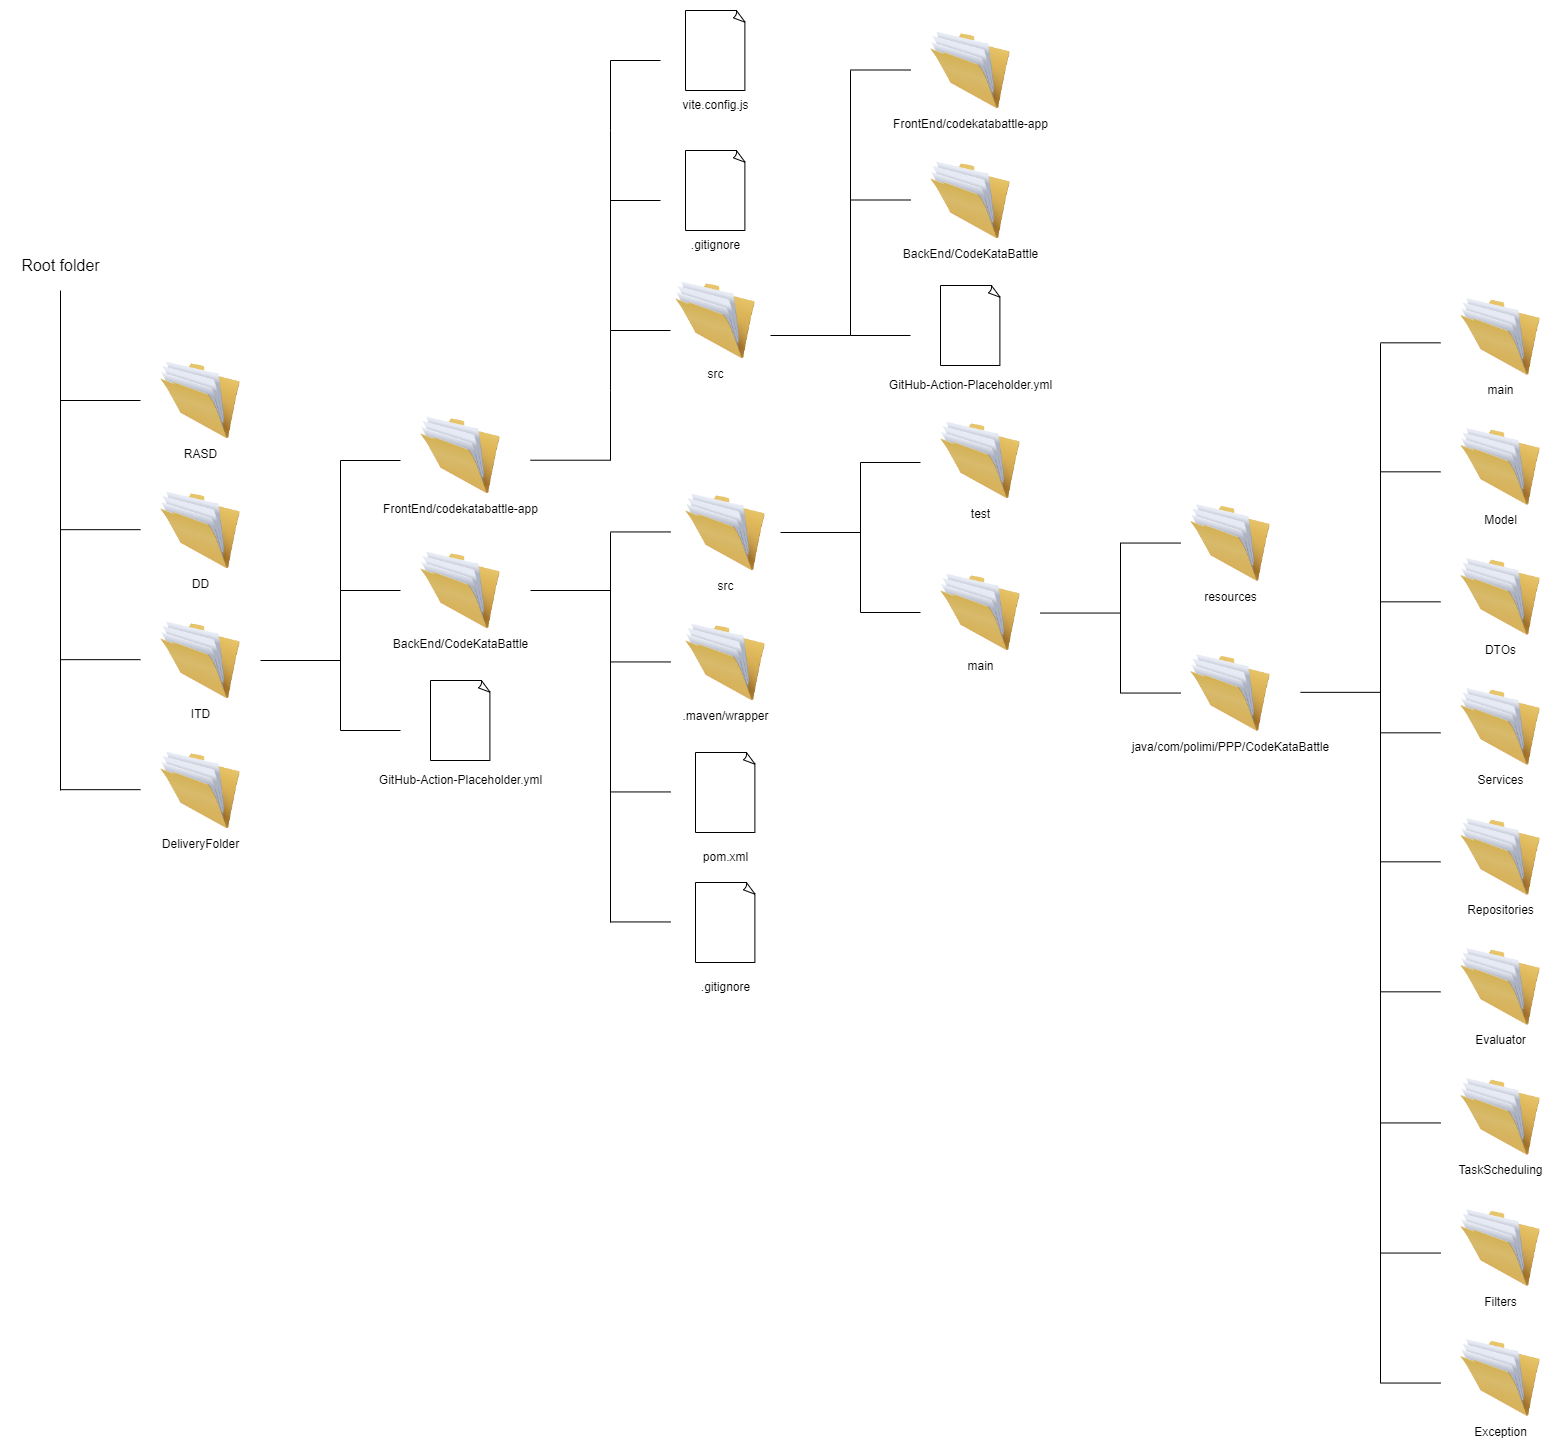
\includegraphics[scale = 0.25]{ITD_latex/Images/SourceCodeStructure.png}
    \caption{Structure of the source code}
\end{figure}

{\color{bluepoli}\rule{\linewidth}{0.1pt}}

% FIFTH CHAPTER
% --------------------------------------------------------------------------
\chapter{Testing}

During the testing phase, we ensured the reliability and functionality of our system.

First, we conducted unit testing on services to deeply examine the business logic. To achieve this, we employed Mockito to mock dependencies for unit tests of components that required dependency injection, focusing on validating the correctness of individual classes, without assessing the correct integration of the components. This step primarily targeted Services.

\begin{figure}[h]
    \centering
    
\includegraphics[scale = 0.25]{ITD_latex/Images/Test/mockito.png}
    \caption{Mockito}
\end{figure}

In the subsequent phase, we conducted comprehensive integration testing using JUnit and MockMVC to simulate requests. To emulate real-world scenarios, we utilized H2, a database management system that is compatible with JPA and operates in memory. This strategy guaranteed that our testing environment closely resembled the production setup, eliminating the need for a separate testing database. Notably, we mocked GitHub APIs and the Email Provider to reduce email spam and avoid exceeding GitHub's API request limits.

The testing process included a total of 39 tests, covering various aspects of the system. Furthermore, we thoroughly tested each endpoint using Postman to ensure the overall robustness and reliability of our application.

\section{Relevant Test Cases}

As mentioned, the entire backend of our application was subjected to exhaustive testing.

\section{Outcomes}

The outcome of our testing process are illustrated below.\\

\begin{figure}[h]
    \centering
    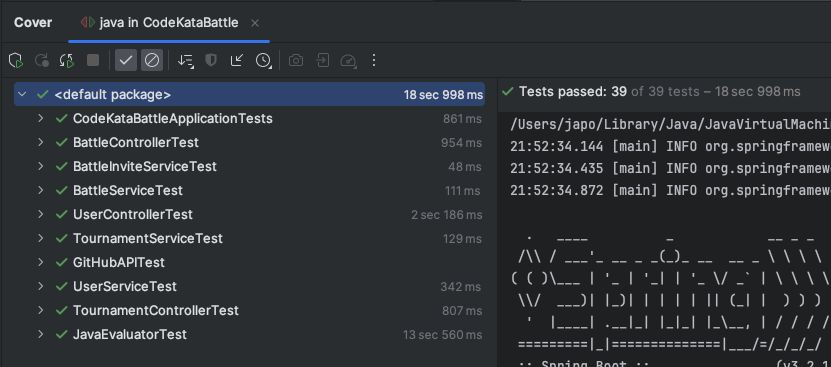
\includegraphics[scale = 0.4]{ITD_latex/Images/Test/Test1.jpg}
    \caption{Test outcome}
\end{figure}

\begin{figure}[h]
    \centering
    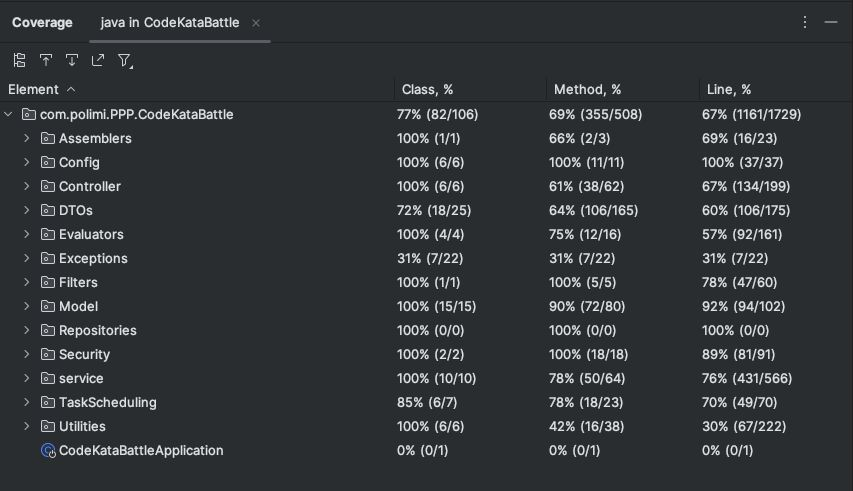
\includegraphics[scale = 0.4]{ITD_latex/Images/Test/Test2.jpg}
    \caption{Test coverage}
\end{figure}

{\color{bluepoli}\rule{\linewidth}{0.1pt}}

% SIXTH CHAPTER
% --------------------------------------------------------------------------
\chapter{Installation guide}

Both the frontend and the backend are already hosted on DigitalOcean.
There is no need of installing anything locally.

The applications are hosted at the following link:

\begin{itemize}
\item \textcolor{bluepoli}{Frontend:} https://codekatabattle.it
\item \textcolor{bluepoli}{CKB:} https://codekatabattle.it:8443
\end{itemize}

{\color{bluepoli}\rule{\linewidth}{0.1pt}}

% SEVENTH CHAPTER
% --------------------------------------------------------------------------
\chapter{Effort spent}

This section shows the amount of time that each member has spent to produce the document. Please notice that each unit is the result of coordinated work among all the members.

\begin{table}[h]
\centering
\begin{tabularx}{\textwidth}{| X | X | X |}
\hline
\textbf{UNIT} & \textbf{MEMBERS} & \textbf{HOURS} \\ [1ex]
\hline
BackEnd & Piazzalunga, Piccinato, Puglisi & 120h \\ [1ex]
\hline
FrontEnd & Puglisi, Piazzalunga, Piccinato & 80h \\ [1ex]
\hline
Testing & Piazzalunga, Puglisi& 20h \\ [1ex]
\hline
Report & Piccinato & 10h \\ [1ex]
\hline
\end{tabularx}
\end{table}

{\color{bluepoli}\rule{\linewidth}{0.1pt}}

% EIGHTH CHAPTER
% --------------------------------------------------------------------------
\chapter{References}

\section{References and Tools}

\begin{enumerate}
    \item GitHub: https://www.github.com
    \item GitHub Actions: https://github.com/features/actions
    \item Diagrams have been made with: http://draw.io
    \item React: https://en.wikipedia.org/wiki/React\_(software)
    \item Spring: https://en.wikipedia.org/wiki/Spring\_Framework
    \item JPA: https://en.wikipedia.org/wiki/Jakarta\_Persistence
    \item Hibernate: https://en.wikipedia.org/wiki/Hibernate\_(framework)
    \item JWT: https://en.wikipedia.org/wiki/JSON\_Web\_Token
    \item DigitalOcean: https://www.digitalocean.com/github-students
\end{enumerate}

{\color{bluepoli}\rule{\linewidth}{0.1pt}}

\end{document}
